
\chapter{Fundamentals} \label{cha:fundamentals}

This chapter summarizes the fundamentals of regression. Excellent overviews can be found in the textbooks \cite{fahrmeir2007regression}, \cite{friedman2001elements} and \cite{wood2017generalized}. The shown fundamentals are strongly aligned with the presentation given in \cite{fahrmeir2007regression}.~\pref{sec:LinModel} gives an overview of the model assumptions used throughout this work. Furthermore,~\pref{sec:ModelSelection} outlines methods to evaluate and compare different models against each other in terms of complexity and accuracy.~\pref{sec:Splines} is devoted to the  spline definitions.

\section{Linear Models} \label{sec:LinModel}
%%%%%%%%%%%%%%%%%%%%%%%%%%%%%%%%%%%%%%%%%%%%%%%%%%%%%%%%%%%%%%%%%%%%%%%%%%%%%%%%%%%%%%%%%%%%%%%%%%%%%%%%%%%%%%%%%%

Given the data set $\mathcal{D} = \{(x^{(i)}_1, \dots, x^{(i)}_q, y^{(i)}), \ i=1,2, \dots, n\}$ comprising $n$ data points, we aim to model the relation between the $q$ inputs $x_1, \dots, x_q$ and the output $y$ with a deterministic function $f(x_1, \dots, x_q)$. Since we cannot assume that the relationship between the inputs and the output is exact, we will include a random part $\epsilon$, which is used to model e.g. measurement errors. It is typically assumed that this part is additive and thus  

\begin{align} \label{eq:model-structure}
	y = f(x_{1}, \dots, x_{q}) + \epsilon.
\end{align}
%
We would like to estimate the unknown function $f(x_1, \dots, x_q)$. For this, some assumptions on the model structure are made:

\begin{enumerate}
	\item \emph{The unknown function $f$ is a linear combination of the inputs}
	
	The function $f(x_1, \dots, x_q)$ is modeled as a linear combination of inputs, i.e. 
	
	\begin{align} \label{eq:linCombOfInputs}
		f(x_1, \dots, x_q) = \beta_0 + \beta_1 x_1 + \dots + \beta_q x_q,
	\end{align}
	
	with unknown parameters $\beta_0, \dots, \beta_q$. Note that the model~\pref{eq:linCombOfInputs} is linear in its parameters as well as in its inputs. The parameter $\beta_0$ is called intercept or bias in the machine learning community, see \cite{bishop2006patternRecognition}. We introduce the input vector $\transpose{\vec{x}} = [1, x_1, \dots, x_q] \in \mathbb{R}^{1 \times q+1}$ and the parameter vector $\transpose{\vec{\beta}} = [\beta_0, \beta_1, \dots, \beta_q] \in \mathbb{R}^{1 \times q+1}$ to obtain 
	\begin{align}
		f(x_1, \dots, x_q) = \transpose{\vec{x}} \vec{\beta}.
	\end{align}
	\newpage
		
	\item \emph{Additive errors}
	
	An additional assumption of linear models is additivity of errors, which means that	
	\begin{align} \label{eq:linModelOneDim}
		y = \transpose{\vec{x}} \vec{\beta} + \epsilon.
	\end{align}
	%
	This is reasonable for many practical applications, even though it appears quite restrictive. 
\end{enumerate}
%
To estimate the unknown parameters or coefficients $\vec{\beta}$, we define the output vector $\transpose{\vec{y}} = [y^{(1)}, \dots, y^{(n)}] \in \mathbb{R}^{1 \times n}$ and the error vector $\transpose{\vec{\epsilon}} = [\epsilon^{(1)}, \dots, \epsilon^{(n)}] \in \mathbb{R}^{1 \times n}$ as well as the design matrix  

\begin{align} \label{eq:design-matrix}
	\vec{X} = \begin{bmatrix}   1     & x^{(1)}_1 & \dots & x^{(1)}_q \\ 
								  	  \vdots & \vdots       &       & \vdots \\ 
				  		  		1     & x^{(n)}_1 & \dots & x^{(n)}_q  
		\end{bmatrix} \in \mathbb{R}^{n \times q+1}		
\end{align}
%
and generate $n$ equations like~\pref{eq:linModelOneDim}, which can be combined to 

\begin{align} \label{eq:LinearModel}
	\vec{y} = \vec{X}\vec{\beta} + \vec{\epsilon}.
\end{align}
%
We assume that the design matrix $\vec{X}$ has full column rank, i.e. $\mathrm{rank}(\vec{X}) = q + 1$, implying linear independence of the columns of $\vec{X}$, which is necessary to obtain a unique estimator for the regression coefficients $\vec{\beta}$, see \cite{fahrmeir2007regression}.

Another necessary requirement is that the number of data points $n$ is larger or equal to the number of regression parameters $p=q+1$, which is equivalent to the statement that the linear system in~\pref{eq:LinearModel} is not underdetermined.

In addition to the assumptions on the unknown function $f$, the necessary assumptions on the error vector $\vec{\epsilon}$ are \cite{fahrmeir2007regression}:

\begin{enumerate}
	\item \emph{Expectation of the error} \\
	The errors have a mean value of zero, i.e. $\text{E}(\vec{\epsilon}) = \vec{0}$.

	\item \emph{Variances and correlation structure of the errors} \\
	We assume constant error variance with $\text{Var} (\epsilon^{(i)}) = \sigma^2$ for $i=1,2,\dots,n$. This property is called homoscedasticity. Additionally, we assume that the errors are uncorrelated, which means $\text{Cov} (\epsilon^{(i)}, \epsilon^{(j)}) = 0$ for $i \ne j$. The combination of these assumptions lead to the covariance matrix $\text{Cov}(\vec{\epsilon}) = \text{E} (\vec{\epsilon} \transpose{\vec{\epsilon}}) = \sigma^2 \vec{I}$.
	
	\item \emph{Assumptions on the input and design matrix} \\
	We have to distinguish two cases where the inputs are deterministic or stochastic. In most cases, the inputs and the output are stochastic and hence all model assumptions are conditioned on the design matrix~\pref{eq:design-matrix}. This means that the input $\vec{x}^{(i)}$ and the errors $\epsilon^{(i)}$ are not stochastically independent. For notational simplicity, we usually suppress the dependence on the design matrix.

	\item \emph{Gaussian errors} \\
	The errors follow at least approximately a normal distribution. Together with Assumption 1 and 2, we obtain that $\epsilon^{(i)} = \mathcal N(0, \sigma^2)$ holds. 
\end{enumerate}
%
Summarizing, we have the following model assumptions:

\begin{equation} \label{eq:lin-model-mean}
	\vec{\mu} = \text{E}(\vec{y}) = \vec{X} \vec{\beta} \\
\end{equation}
\begin{equation} \label{eq:lin-model-var}
	\text{Cov} (\vec{y}) = \sigma^2 \vec{I}, \\
\end{equation}
%	
yielding 

\begin{equation} \label{eq:linModelAsDistribution}
	\vec{y} \sim \mathcal N(\vec{X} \vec{\beta}, \sigma^2 \vec{I}).
\end{equation}
%
A linear model with multiple inputs can therefore be interpreted as a multi-variate normal distribution with its mean vector given by~\pref{eq:lin-model-mean} and its covariance matrix given by~\pref{eq:lin-model-var}. To specify the linear model given in~\pref{eq:linModelAsDistribution}, we need to estimate the regression coefficients $\vec{\beta}$ and the variance $\sigma^2$.

%%%%%%%%%%%%%%%%%%%%%%%%%%%%%%%%%%%%%%%%%%%%%%%%%%%%%%%%%%%%%%%%%%%%%%%%%%%%%%%%%%%%%%%%%%%%%%%%%%%%%%%%%%%%%%%%%%
\subsection{Estimation of the Regression Parameters \texorpdfstring{$\vec{\beta}$}{TEXT}}

The linear model given in~\pref{eq:linModelAsDistribution} features the unknown parameters $\vec{\beta}$ and $\sigma^2$, which need to be estimated using the given data $\mathcal{D}$. In the following, the estimator $\hat{\vec{\beta}}$ is introduced. The two methods to estimate the regression parameters in the context of linear models are the method of Least Squares (LS) and the method of Maximum Likelihood (ML).  

\subsubsection{The Method of Least Squares} \label{subsubsec:Method-of-LS}

The unknown regression parameters $\vec{\beta} \in \mathbb{R}^p$ are estimated by minimizing the sum of squared error

\begin{align} \label{eq:MethodOfLS} 
	\text{LS}(\vec{y}, \vec{\beta}) &=  \lVert \vec{y} - \vec{X} \vec{\beta} \rVert^2_2 = \sum_{i=1}^n\epsilon_i^2 = \transpose{\vec{\epsilon}} \vec{\epsilon},
\end{align}
%
with respect to $\vec{\beta}$, see, e.g. \cite{friedman2001elements}. Rewriting~\pref{eq:MethodOfLS} leads to the least squares criterion

\begin{align} \label{eq:LS_derivation}
		\begin{split}
				\text{LS}(\vec{y}, \vec{\beta})  &=\transpose{(\vec{y} - \vec{X} \vec{\beta})}(\vec{y} - \vec{X} \vec{\beta}) \\ 
								 				&=\transpose{\vec{y}}\vec{y} - 2\transpose{\vec{y}}\vec{X} \vec{\beta} + \transpose{\vec{\beta}}    \transpose{\vec{X}} \vec{X} \vec{\beta}.
		\end{split}
\end{align}
%
The first-order necessary condition for optimality, cf. \cite{luenberger1984linear}, reads as

\begin{align} \label{eq:LS_1st_derivative}
	\frac{\partial \text{LS}(\vec{y}, \vec{\beta})}{\partial \vec{\beta}} = -2\transpose{\vec{X}} \vec{y} + 2 \transpose{\vec{\beta}} \transpose{\vec{X}} \vec{X} = 0.
\end{align}
%
The second-order condition for optimality requires the Hessian, i.e. 

\begin{align} \label{eq:LS_2nd_derivative}
	\frac{\partial^2 \text{LS}(\vec{y}, \vec{\beta})}{\partial \vec{\beta} \partial \transpose{\vec{\beta}}} = 2\transpose{\vec{X}}\vec{X},
\end{align}
to be positive-definite. Since the design matrix $\vec{X} \in \mathbb{R}^{n \times p}$ is assumed to have full rank, the matrix $ \transpose{\vec{X}}\vec{X}$ is positive-definite. The least squares estimate $\hat{\vec{\beta}}_{LS}$ is hence obtained, see~\pref{eq:LS_1st_derivative}, by solving the so-called \emph{normal equations}

\begin{align} \label{eq:NormalEquations}
	\transpose{\vec{X}} \vec{X} \vec{\beta} = \transpose{\vec{X}} \vec{y}.
\end{align}
%
Since $\transpose{\vec{X}}\vec{X}$ is positive-definite, the \emph{normal equations}~\pref{eq:NormalEquations} feature a unique solution given by the least squares estimator

\begin{align} \label{eq:LS_estimator}
	\hat{\vec{\beta}}_{\mathrm{LS}} = (\transpose{\vec{X}}\vec{X})^{-1} \transpose{\vec{X}}\vec{y}.
\end{align}

\subsubsection{Maximum Likelihood Estimation}

Under the normality assumption and given the data $\mathcal{D}$, the likelihood is defined, see \cite{wood2017generalized}, as

\begin{align} \label{eq:likelihood}
	\mathcal{L}(\vec{\beta}, \sigma^2) = \frac{1}{(2\pi\sigma^2)^{n/2}} \exp \left( -\frac{1}{2\sigma^2}\transpose{(\vec{y} - \vec{X} \vec{\beta})}(\vec{y} - \vec{X} \vec{\beta}) \right).
\end{align}
%
The log-likelihood is then given by taking the logarithm of~\pref{eq:likelihood} as

\begin{align} \label{eq:log_liklihood}
	l(\vec{\beta}, \sigma^2) = -\frac{n}{2}\log(2\pi) - \frac{n}{2}\log(\sigma^2) - \frac{1}{2\sigma^2}\transpose{(\vec{y} - \vec{X} \vec{\beta})}(\vec{y} - \vec{X} \vec{\beta}).
\end{align}
%
Thus, maximizing the log-likelihood $l(\vec{\beta}, \sigma^2)$ with respect to $\vec{\beta}$ is equivalent to minimizing the least squares criterion given in~\pref{eq:MethodOfLS}. The maximum likelihood estimator $\hat{\vec{\beta}}_{\mathrm{ML}}$ is therefore equivalent to the least squares estimator $\hat{\vec{\beta}}_{\mathrm{LS}}$ in~\pref{eq:LS_estimator}.

%%%%%%%%%%%%%%%%%%%%%%%%%%%%%%%%%%%%%%%%%%%%%%%%%%%%%%%%%%%%%%%%
\subsection{Estimation of the Variance $\sigma^2$}

The estimation of the variance $\sigma^2$ is necessary for the construction of confidence intervals of the regression parameters and for the construction of prediction intervals. It is further used in all kinds of statistical tests as well as in model selection approaches and model assessment criteria \cite{blobel2013statistische}.

\subsubsection{Maximum Likelihood Estimation}

The first-order necessary condition for optimality in this case yields 

\begin{align} \label{eq:log_likelihood_derivative_sigma}
	\frac{\partial l(\vec{\beta}, \sigma^2)}{\partial \sigma^2} = -\frac{n}{2\sigma^2} + \frac{1}{2\sigma^4}\transpose{(\vec{y} - \vec{X} \vec{\beta})}(\vec{y} - \vec{X}\vec{\beta}) = 0. 
\end{align}
%
Substituting the maximum likelihood estimator $\hat{\vec{\beta}}_{\mathrm{ML}}$, note the equivalence with the least squares estimator $\hat{\vec{\beta}}_{\mathrm{LS}}$ given in~\pref{eq:LS_estimator}, for $\vec{\beta}$ results in the maximum likelihood estimator 

\begin{align} \label{eq:sigma_ML}
	\hat \sigma^2_{ML} = 
		\frac{(\vec{y} - \vec{X} \transpose{\hat{\vec{\beta}}_{\mathrm{LS}})}(\vec{y} - \vec{X} \hat{\vec{\beta}}_{\mathrm{LS}})}{n} = \frac{1}{n} \transpose{\hat{\vec{\epsilon}}} \hat{\vec{\epsilon}}
\end{align}
%
where $\hat{\vec{\epsilon}}$ is the estimate of the error $\vec{\epsilon}$. This estimator for $\sigma^2$ is rarely used since it is biased, i.e. $\text{E}(\hat \sigma^2_{\mathrm{ML}}) \ne \sigma^2$, see \cite{fahrmeir2007regression}. 

\subsubsection{Restricted Maximum Likelihood Estimation}

The mean value of the sum of squared residuals is $\text{E}(\transpose{\hat{\vec{\epsilon}}} \hat{\vec{\epsilon}}) = (n - p)\sigma^2$. Hence, another estimator for $\sigma^2$ is given by

\begin{align} \label{eq:sigma_REML}
	\hat \sigma^2_{\mathrm{REML}} = \frac{1}{n-p} \transpose{\hat{\vec{\epsilon}}} \hat{\vec{\epsilon}}.
\end{align}
%
The restricted maximum likelihood estimator (REML) $\hat \sigma^2_{\mathrm{REML}}$ is in general less biased \cite{fahrmeir2007regression}. Therefore, it is the commonly used estimator for the variance $\sigma^2$.

%%%%%%%%%%%%%%%%%%%%%%%%%%%%%%%%%%%%%%%%%%%%%%%%%%%%%%%%%%%%%%%%%%%%%%%%%%%%%%%%%%%%%%%%%%%%%%%%%%%%%%%%%%%%%%%%%%
\subsection{The Hat Matrix} \label{subsec:Hat-Matrix}

Using the least squares estimator~\pref{eq:LS_estimator}, we can estimate the mean of $\vec{y}$ by 

\begin{align} \label{eq:mean_of_y}
	\widehat{\text{E}(\vec{y})} = \vec{\hat{y}} = \vec{X} \hat{\vec{\beta}}_{\mathrm{LS}}.
\end{align}
%
Substituting $\hat{\vec{\beta}}_{\mathrm{LS}}$ in~\pref{eq:mean_of_y} by~\pref{eq:LS_estimator} results in 
%
\begin{align} \label{eq:hat-matrix}
	\vec{\hat{y}} =  \vec{H} \vec{y},
\end{align}
%
with the matrix
%
\begin{align} \label{eq:hat-matrix-def}
	\vec{H} = \vec{X}(\transpose{\vec{X}} \vec{X})^{-1} \transpose{\vec{X}} \in \mathbb{R}^{n \times n}, 
\end{align}
%
which is called \emph{hat matrix}, cf.~\cite{fahrmeir2007regression}. Using the hat matrix $\vec{H}$, we can express the residuals $\hat \epsilon^{(i)} = y^{(i)} - \hat y^{(i)}$ in matrix notation as

\begin{align} \label{eq:residal_with_hat_matrix}
	\hat{\vec{\epsilon}} = \vec{y} - \hat{\vec{y}} = (\vec{I} - \vec{H}) \vec{y}.
\end{align}
%
The hat matrix $\vec{H}$ has the following useful properties:

\begin{itemize}
	\item $\vec{H}$ is symmetric.
	\item $\vec{H}$ is idempotent, i.e. $\vec{H}^2 = \vec{H}$.
	\item The rank of $\vec{H}$ is equal to its trace.
 	\item $\frac{1}{n} \le h_{ii} \le 1$, if all data points are different, i.e. $x^{(i)} \ne x^{(j)}$ for $i \ne j$. Here, $h_{ii}$ are the diagonal elements of $\vec{H}$.
	\item The matrix $(\vec{I} - \vec{H})$ is also idempotent and symmetric, with $\mathrm{rank}(\vec{I} - \vec{H}) = n - p$.
\end{itemize}

The hat matrix $\vec{H}$ is used in model selection techniques like cross-validation since its trace acts as a measure for the degrees of freedom of the model, as well as in outlier detection and in diagnostic plots for linear models. Note that the trace of the hat matrix $\vec{H}$ is equal to the number of parameters for linear models. 

%%%%%%%%%%%%%%%%%%%%%%%%%%%%%%%%%%%%%%%%%%%%%%%%%%%%%%%%%%%%%%%%%%%%%%%%%%%%%%%%%%%%%%%%%%%%%%%%%%%%%%%%%%%%%%%%%%
\section{Model Selection} \label{sec:ModelSelection}

Linear models are widely exploit for regression problems on large data sets $(n \gg 1)$, because the solution of the \emph{normal equations}~\pref{eq:NormalEquations} can be computed efficiently even for large $n$. If these data sets also contain a large number of inputs $(q \gg 1)$, the situation becomes more complicated since possible interaction effects or correlation of input variables may occur. These interaction terms limit the, otherwise perfect, interpretability of the linear model. 

Therefore, we need techniques and criteria to select the \emph{best possible model} out of the variety of different models for a given data set. Model assessment criteria, see Section~\pref{subsec:MAC}, are used to compare different models while subset selection techniques, see Section~\pref{subsec:SSM}, give an algorithmic approach to model generation. Furthermore, we can influence the estimated coefficients $\vec{\beta}$ directly via regularization, see Section~\pref{subsec:Regularization}. 

%%%%%%%%%%%%%%%%%%%%%%%%%%%%%%%%%%%%%%%%%%%%%%%%%%%%%%%%%%%%%%%%
\subsection{Model Assessment Criteria} \label{subsec:MAC}

One way of comparing various models, i.e. models using different sets of inputs, is the use of model assessment criteria. Generally, model assessment criteria can be split in two components. The first one measures the quality of fit, e.g., using the sum of squared errors, while the second measures the complexity of the model. Most model assessment criteria are based on the sum of the expected squared prediction error (SPSE), which is also known as \emph{generalization error}. Therefore, the derivation of the SPSE is given next. 

\subsubsection{Sum of Expected Squared Prediction Error} \label{subsubsec:SPSE}

Given independent observations $y^{(i)}, \ i=1,2, \dots, n$ and a subset of $q$ inputs $\{x_0=1, x_1, x_2, \dots, x_q\}$, we want to measure the prediction quality. The specific models are defined
by numbers $M \subset \{1, \dots, p\}$ of used inputs with corresponding design matrix $\vec{X}_M$. Moreover, $\vert M \vert$ is the cardinal number of $M$, i.e. the number of inputs included in the model. The least squares estimator for $\vec{\beta}$, cf.~\pref{eq:LS_estimator}, is then given by

\begin{align*}
	\hat{\vec{\beta}}_{M} = (\transpose{\vec{X}}_M \vec{X}_M)^{-1} \transpose{\vec{X}}_M \vec{y}.
\end{align*}
%
The data $\vec{y}$ can be interpreted as a random variable. We can then define an estimator $\hat{\vec{y}}_M$ for the vector $\vec{\mu}$ of expectations $\mu^{(i)} = \text{E}(y^{(i)})$ as

\begin{align} \label{eq:SPSE-estimator-y}
	\vec{\hat{y}}_M = \vec{X}_M  \hat{\vec{\beta}}_M.
\end{align}
%
Moreover, it is easy to show that the following properties hold true using the hat matrix $\vec{H}_M = \vec{X}_M (\transpose{\vec{X}}_M \vec{X}_M)^{-1}\transpose{\vec{X}}_M$ defined in~\pref{eq:hat-matrix-def}:

\begin{enumerate}[(i)]%
	\item $\text{E} (\vec{\hat{y}}_M) = \vec{H}_M \text{E}(\vec{y})$ 
	\item $\text{Cov} (\vec{\hat{y}}_M) = \sigma^2 \vec{H}_M$
	\item $\sum_{i=1}^n \text{Var}(\hat y^{(i)}_M) =  \text{trace}(\vec{H}_M) \sigma^2 = \vert M \vert \sigma^2 $
	\item Sum of Mean Squared Error
		\begin{equation} 
		\begin{split} 
		\text{SMSE} &= \sum_{i=1}^n \text{E}\left(\hat y^{(i)}_M - \mu^{(i)}\right)^2 \\
				    &= \sum_{i=1}^n \text{E}\left( \big( \hat y^{(i)}_M - \text{E}(\hat y^{(i)}_M) \big) + \big(\text{E}(\hat y^{(i)}_M) - \mu^{(i)} \big) \right)^2 \\
				    &= \vert M \vert\sigma^2 + \sum_{i=1}^n \left( \text{E}(\hat y^{(i)}_M) - \mu^{(i)} \right)^2.
		\end{split}
		\end{equation}
\end{enumerate}

Note that the estimator~\pref{eq:SPSE-estimator-y} can be regarded as a prediction for future observations of the form

\begin{align}
	y^{(n+i)} = \mu^{(i)} + \epsilon^{(n+i)}
\end{align}
%
for new input data $\{(x_1^{(i)}, \dots, x_q^{(i)}), i=1,2,\dots,n\}$. Thus, we can derive the SPSE as

\begin{equation}
\begin{split}
	\text{SPSE} &= \sum_{i=1}^{n} \text{E}\left(y^{(n+i)} - \hat y^{(i)}_M\right)^2 \\ 
				&= \sum_{i=1}^{n} \text{E}\left((y^{(n+i)} - \mu^{(i)}) - (\hat y^{(i)}_M - \mu^{(i)})\right)^2 \\ 
				&= \sum_{i=1}^{n} \text{E}\left(y^{(n+i)} - \mu^{(i)}\right)^2 + 2\text{E} \left( (y^{(n+i)} - \mu^{(i)})(\hat y^{(i)}_M - \mu^{(i)}) \right) + \text{E}\left(\hat y^{(i)}_M - \mu^{(i)}\right)^2 \\
				&= \sum_{i=1}^{n}\text{E}\left(y^{(n+i)} - \mu^{(i)}\right)^2 + \sum_{i=1}^{n} \text{E}\left( \hat y^{(i)}_M - \mu^{(i)} \right)^2 \\ 
				&= n\sigma^2 + \text{SMSE} \\ 
				&= n\sigma^2 + \vert M \vert \sigma^2 + \sum_{i=1}^{n} \left(\text{E}(\hat y^{(i)}_M) - \mu^{(i)} \right)^2.
\end{split}
\end{equation}

The SPSE can be split into three parts:

\begin{enumerate}
	\item \emph{Irreducible Prediction Error Term}: $n\sigma^2$ \\
	This term cannot be reduced through model selection techniques since it only contains the number of data points $n$ and the variance $\sigma^2$.

	\item \emph{Variance Error Term}: $\vert M \vert \sigma^2$ \\
	The second term contains the number of used variables $\vert M \vert$ as well as the variance $\sigma^2$. It can therefore be reduced by reducing the model complexity, i.e. by using a smaller number of inputs.
	
	\item \emph{Squared Bias Error Term}: $\sum_{i=1}^{n} \left( \text{E}(\hat y^{(i)}_M) - \mu^{(i)} \right)^2$\\
	The last term can be interpreted as bias. It can be reduced by increasing the model complexity, i.e. by using additional inputs.
\end{enumerate}
%
The SPSE acts as an example of the bias-variance trade-off, which is characteristic for all statistical models. It states that by increasing the model complexity, the bias is reduced but instead the variance is increased. On the other hand, by decreasing model complexity, the variance of the model is reduced, but the bias is increased, see~\pref{fig:bv-trade-off} and \cite{bishop2006patternRecognition}.

\begin{figure}[H]
	\centering
	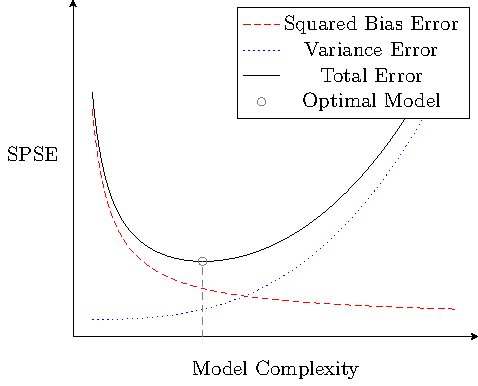
\includegraphics{graphics/pgfplots/cha2/bvd.pdf}
	\caption{Bias-variance trade-off.}
	\label{fig:bv-trade-off}
\end{figure}
%
In practice, the true value for the SPSE is not accessible since $\mu^{(i)}$ and $\sigma^2$ are unknown. Therefore, we need to estimate the SPSE. This can be done by using one of the following two strategies:

\begin{enumerate}

	\item \emph{Estimate SPSE using new and independent data} \\	
	If new observations are available, the SPSE can be estimated by
	\begin{align}
		\widehat{\text{SPSE}} = \sum_{i=1}^n \left(y^{(n+i)} - \hat y^{(i)}_M\right)^2.
	\end{align}
	These new observations can also be some held-out validation data from a train-validation split of the given data. 
	
	\item \emph{Estimate SPSE using existing data} \\
	When using existing data, the estimate for the SPSE is given by the squared error and an additional  term depending on the estimated variance and the model complexity. The estimate is thus given by
	\begin{align}
		\widehat{\text{SPSE}} = \sum_{i=1}^n \left(y^{(i)} - \hat y^{(i)}_M\right)^2 + 2\vert M \vert \hat \sigma^2.
	\end{align}

\end{enumerate}

Typically used model assessment criteria follow the basic idea of the SPSE, see \cite{fahrmeir2007regression}.

\subsubsection{Mean Squared Error} 

The mean squared error MSE is one of the standard metrics for regression and defined as

\begin{align} \label{eq:MSE-DEF}
	\mathrm{MSE} = \frac{1}{n} \sum_{i=1}^n \left(y^{(i)} - \hat y^{(i)}_M \right),	
\end{align}
%
where $y^{(i)}$ is the given data and $\hat y^{(i)}_M$ is the model prediction for that point. 

\subsubsection{Corrected Coefficient of Determination $\text{R}_{\mathrm{corr}}^2$}

The corrected coefficient of determination $\text{R}^2_{\mathrm{corr}}$ is an improvement over the coefficient of determination $\text{R}^2$, which is defined as 

\begin{align}
	\text{R}^2 = 1 - \frac{\sum_{i=1}^n \left( y^{(i)} - \hat y^{(i)}_M \right)^2}{\sum_{i=1}^n \left(y^{(i)} - \bar y\right)^2},
\end{align}
%
where $\bar y$ is the mean value of $\vec{y}$. The major drawback of $\text{R}^2$ is that it will never decrease when further inputs are included in the model, e.g. the $\text{R}^2$ of a model using $\{x_1, x_2, x_3\}$ is always larger or equal the $\text{R}^2$ of a model using $\{x_1, x_2\}$, even if the variable does not enhance the prediction quality. 

The corrected coefficient of determination $\text{R}_{\mathrm{corr}}^2$ reduces this problem by an correction term depending on the  number of parameters and is given by
\begin{align}
	\text{R}_{\mathrm{corr}}^2 = 1 - \frac{n-1}{n-p}(1-\text{R}^2).
\end{align}

The corrected coefficient of determination is a standard output parameter in many statistical programs and may be used to compare even models with different number of used variables \cite{fahrmeir2007regression}.

\subsubsection{Corrected Coefficient of Determination after McFadden $\text{R}_{\mathrm{McFadden}}^2$}

The corrected coefficient of determination after McFadden is defined as

\begin{align}
	\text{R}_{\mathrm{McFadden}}^2 = 1 - \frac{\ln{(\mathcal{L}_M)} - \vert M \vert }{\ln{(\mathcal{L}_0)}}
\end{align}
%
using the likelihood of the model $M$ given by $\mathcal{L}_M$ and the likelihood of the zero model $\mathcal{L}_0$. A standard zero model is given by the mean value $\bar y$. Higher values of $\text{R}_{\mathrm{McFadden}}^2$ correspond to better fits.

\subsubsection{Mallow's $\mathbf{C_p}$}

Mallow's complexity parameter is based directly on the ideas specified for the estimation of the SPSE and is given by

\begin{align}
	\text C_\mathrm{p} = \frac{\sum_{i=1}^n \left(y^{(i)} - \hat y^{(i)}_M\right)^2}{\hat \sigma^2} - n + 2 \vert M \vert.
\end{align}
%
A lower value of Mallow's $\text C_\mathrm{p}$ corresponds to a better model fit \cite{fahrmeir2007regression}.

\subsubsection{Akaike Information Criterion}

The AIC is among the most used model assessment criteria and defined by

\begin{align}
	\text{AIC} = -2 l(\hat{\vec{\beta}}_{\mathrm{ML}}, \hat \sigma^2_{\mathrm{ML}}) + 2(\vert M \vert +1),
\end{align}
%
where $l(\hat{\vec{\beta}}_{\mathrm{ML}}, \hat \sigma^2_{\mathrm{ML}})$ is the value of the log-likelihood~\pref{eq:log_liklihood} at its maximum, i.e. at $\hat{\vec{\beta}}_{\mathrm{ML}}$ and $\hat{\sigma}_{\mathrm{ML}}$. It is worth noting that the total number of parameters is $\vert M \vert + 1$ because the variance is also counted as parameter. The log-likelihood for a linear model assuming Gaussian errors is given by, cf.~\pref{eq:log_liklihood},

\begin{align}
	-2l(\hat{\vec{\beta}}_{\mathrm{ML}}, \hat \sigma_{\mathrm{ML}}^2) = n \log(\hat \sigma_{\mathrm{ML}}^2) + n.
\end{align}
%
Therefore, neglecting the constant $n$, the AIC evaluates to

\begin{align}
	\text{AIC} = n \log(\hat \sigma^2_{\mathrm{ML}}) + 2(\vert M \vert + 1).
\end{align}
%
A lower value of the AIC corresponds a to a better model fit \cite{fahrmeir2007regression}.

\subsubsection{Bayesian Information Criteria}

The BIC is similar to the AIC, but it penalizes more complex models much harder than the AIC. In its general form, it is given as 

\begin{align}
	\text{BIC} = -2l(\hat{\vec{\beta}}_{\mathrm{ML}}, \hat \sigma^2_{\mathrm{ML}}) + \log(n) (\vert M \vert + 1).
\end{align}
%
Again, assuming Gaussian errors for a linear model and neglecting the constant term $n$, the BIC evaluates to

\begin{align}
	\text{BIC} = n\log(\hat \sigma_{\mathrm{ML}}^2) + \log(n)(\vert M\vert + 1).
\end{align}
%
A lower value of the BIC correspond to a better model fit \cite{fahrmeir2007regression}.

\subsubsection{Cross-validation} \label{subsubsec:Cross-validation}

The basic idea of cross-validation (CV) is to split the given data set into a training set to estimate the parameters and a validation set to assess the prediction quality. A special case of cross-validation is the "leave-one-out" cross-validation, where all but one data point are used for training and the model is then evaluated on this held-out data point. This seems to be quite expensive, since one needs to estimate one model per data point. However, it can be shown that the cross-validation score can be computed using one model trained on all data $\vec{y}$ and the hat matrix $\vec{H}_M = \vec{X}_M (\transpose{\vec{X}}_M \vec{X}_M)^{-1} \transpose{\vec{X}}_M$, see Section~\pref{subsec:Hat-Matrix}. The cross-validation score is then given by

\begin{align} \label{eq:cross-validation}
	\text{CV} = \frac{1}{n} \sum_{i=1}^n \left( \frac{y^{(i)} - \hat y^{(i)}_M}{1 - h_{ii,M}} \right)^2,
\end{align}
%
where $h_{ii,M}$ denote the diagonal elements of the hat matrix $\vec{H}_M$ and $\hat y^{(i)}_M$ is defined as the prediction of the model $M$ for the input $\{x^{(i)}_1, \dots, x^{(i)}_q \}$. A lower cross-validation score corresponds to a better model fit \cite{golub1979}.

An approximation to the cross-validation score is given by the so-called generalized cross-validation (GCV) score. It is mainly used in the context of non-parametric regression, when the hat matrix $\vec{H}_M$ is numerically expensive to compute or when regularization, see Section~\pref{subsec:Regularization}, is applied. In the GCV score, the diagonal elements of the hat matrix $h_{ii,M}$ are replaced by the mean of the trace of $\vec{H}_M$. The GCV score is then given by

\begin{align} \label{eq:generalizied-cross-validation}
	\text{GCV} = \frac{1}{n}\sum_{i=1}^n \left( \frac{y^{(i)} - \hat y^{(i)}_M}{1 - \text{trace}(\vec{H}_M)/n}\right)^2.
\end{align}
%
The numerical advantage comes from the fact that the trace of a product of matrices is invariant to cyclical permutations, i.e.

\begin{align}\label{eq:trace-hat-matrix-cyclical-perm}
	\begin{split}
	\text{trace}(\vec{H}_M) {}&= \text{trace}\left(\vec{X}_M(\transpose{\vec{X}}_M \vec{X}_M)^{-1} \transpose{\vec{X}}_M\right) \\ {}&=\text{trace}\left(\transpose{\vec{X}}_M \vec{X}_M (\transpose{\vec{X}}_M \vec{X}_M)^{-1}\right) = \vert M \vert.
\end{split}
\end{align} 
%
The trace can therefore be computed from the product of two matrices of shape $\vert M \vert\times \vert M \vert$, see  \cite{fahrmeir2007regression}. Note that for a linear model as in~\pref{eq:LinearModel}, the trace of the hat matrix $\vec{H}$ is equal to the number of parameters $p$ of the linear model. For regularized or non-parametric models, the trace of the hat matrix $\vec{H}$ is smaller than $p$, where $p$ is the number of parameters of the regularized or non-parametric model. Therefore, the trace of the hat matrix $\vec{H}$ is also known as \emph{effective degree of freedom} EDoF of the model, see Section~\ref{subsec:Regularization}. 


%%%%%%%%%%%%%%%%%%%%%%%%%%%%%%%%%%%%%%%%%%%%%%%%%%%%%%%%%%%%%%%%
\subsection{Subset Selection Methods} \label{subsec:SSM}

To make use of the various model assessment criteria, some algorithmic approach to model selection needs to be given. The most commonly used approaches are forward, backward and stepwise selction \cite{fahrmeir2007regression}. 

In forward selection, we start with a candidate model, which includes a small number of variables. In each iteration of forward selection, an additional variable is added to the candidate model.  The added variable is the one which leads to the largest reduction of a predefined model assessment criteria. The algorithm stops, if no further reduction is achieved.

In backward selection, we start with a candidate model, which includes all variables. In each iteration of backward selection, we eliminate the variable from the model which elimination provides the largest improvement of a predefined model assessment criteria. The algorithm stops, if no further improvement is possible. 

In step-wise selection, forward and backward selection are combined to enable the inclusion and deletion of a variable in every operation. The algorithm stops, if no further reduction is possible.

%%%%%%%%%%%%%%%%%%%%%%%%%%%%%%%%%%%%%%%%%%%%%%%%%%%%%%%%%%%%%%%%
\subsection{Regularization} \label{subsec:Regularization}

Model selection can also be achieved using regularization techniques by directly influencing the parameters $\vec{\beta}$, which need to be estimated given a data set. In general, regularization restricts the parameter space by adding some penalty term depending on the complexity of the model to the least squares objective function according to~\pref{eq:MethodOfLS}. This leads to the penalized least squares (PLS) criterion

\begin{align} \label{eq:PLS_crit}
	\text{PLS}(\vec{y}, \vec{\beta}; \lambda) = \lVert \vec{y} - \vec{X} \vec{\beta}\rVert^2_2 + \lambda \cdot \text{pen}(\vec{\beta}),
\end{align}
%
where $\lambda$ is the so-called \emph{smoothing parameter} and $\text{pen}(\vec{\beta})$ is the penalty term describing the regularization technique. 

In Ridge regression, the penalty term in the penalized least squares criterion in~\pref{eq:PLS_crit} is given by the squared weighted $L_2$-norm of the parameter vector $\vec{\beta}$, i.e. $\text{pen}(\vec{\beta}) = \lVert \vec{\beta} \rVert^2_{\vec{K}} = \transpose{\vec{\beta}} \vec{K} \vec{\beta}$ with a positive definite penalty matrix $\vec{K} \in \mathbb{R}^{p \times p}$. The closed-form solution reads as

\begin{align}
	\hat{\vec{\beta}}_{\mathrm{PLS}} = \arg \min_{\vec{\beta}} \left(\text{PLS}(\vec{y}, \vec{\beta}; \lambda) \right) = (\transpose{\vec{X}} \vec{X} + \lambda \vec{K})^{-1} \transpose{\vec{X}}\vec{y}.
\end{align}
%
The additional penalty term in Ridge regression leads to smaller parameter estimates $\hat{\vec{\beta}}_{\mathrm{PLS}}$ compared to the unpenalized estimate $\hat{\vec{\beta}}_{\mathrm{LS}}$. For large values of the smoothing parameter $\lambda$, the parameter estimates will converge towards, but never reach, zero. 

Ridge regression is commonly used when the input dimension $q$ is high, i.e. the number of parameters $\vec{\beta}$ is large, and also known as Tikhonov regularization \cite{hoerl1970ridge}. Note that it is also possible to use a penalty matrix $\vec{K}(\vec{\beta})$ resulting in

\begin{align}
	\text{pen}(\vec{\beta}) = \lVert \vec{\beta} \rVert^2_{\vec{K}(\vec{\beta})} = \transpose{\vec{\beta}} \vec{K}(\vec{\beta}) \vec{\beta}.
\end{align}
%
However, the resulting penalized least squares problem  has no closed-form solution and must be solved by an iterative approach. We start with an initial guess $\vec{\beta}^{[0]}$ and compute for $k = 0, 1, 2, \dots$ the iteration

\begin{align} \label{eq:PLS-iterative-approach}
	\vec{\beta}^{[k+1]} = \left(\transpose{\vec{X}} \vec{X} + \lambda \vec{K}(\vec{\beta}^{[k]}) \right)^{-1} \transpose{\vec{X}} \vec{y},
\end{align}
%
until $\left\lVert \vec{\beta}^{[k+1]} - \vec{\beta}^{[k]}  \right\rVert \le \text{Tol}$ with $\text{Tol}$ being a given tolerance. The derivation of the iteration~\pref{eq:PLS-iterative-approach} is presented in~\pref{apx:AppendixB}.

Note that by the introduction of the penalty matrix $\vec{K} \ne \vec{0}$, we reduce the degrees of freedom of the model. This can be seen by comparing the trace of the hat matrix $\vec{H}$ of the regularized model, i.e.

\begin{align} \label{eq:hat-matrix-regularizated-mode}
	\vec{H}_{\mathrm{pen}} = \vec{X} (\transpose{\vec{X}} \vec{X} + \lambda \vec{K})^{-1} \transpose{\vec{X}},
\end{align} 
%
with the trace of the hat matrix of the unpenalized model, see~\pref{eq:hat-matrix}. The trace of the hat matrix $\vec{H}$ is also called \emph{effective degree of freedom}, i.e.

\begin{align} \label{eq:EDoF}
	\text{EDoF} = \text{trace}(\vec{H}_{\mathrm{pen}}).
\end{align}
%
When we use regularization to reduce the degree of freedom of a model, we need to make use of the effective degree of freedom EDoF instead of the number of parameters $p$ in model assessment criteria, see Section~\pref{subsec:MAC}. 

\subsubsection{L-curve method} \label{subsubsec:L-curve}

Another method for choosing the regularization parameter, additional to the model assessment criteria in Section~\pref{subsec:MAC}, is the so-called \emph{L-curve method}. The L-curve is given by the parametric curve $(\rho(\lambda), \eta(\lambda))$, where $\rho(\lambda)$ and $\eta(\lambda)$ measure the size of the regularization $\transpose{\vec{\beta}} \vec{K} \vec{\beta}$ and the residual $\lVert \vec{y} - \vec{X} \vec{\beta} \rVert_2^2$, see \cite{hansen1993use}. In the setting of Ridge regression, this curve then has a distinct L-shaped corner exactly where the solution $\vec{\beta}$ changes from being dominated by the regularization errors $\lambda \cdot \mathrm{pen}(\vec{\beta})$ to being dominated by the mean squared data errors $\lVert \vec{y} - \vec{X} \vec{\beta} \rVert$. This corner determines the smoothing parameter $\lambda$ as optimal trade-off between data fidelity and smoothness. The L-curve method can also be used when the data errors are correlated, a situation in which generalized cross-validation, see~\pref{subsubsec:Cross-validation}, fails to produce the optimal regularization parameter. Further information can be found in \cite{hansen1993use} and \cite{hansen1992analysis}.


%%%%%%%%%%%%%%%%%%%%%%%%%%%%%%%%%%%%%%%%%%%%%%%%%%%%%%%%%%%%%%%%%%%%%%%%%%%%%%%%%%%%%%%%%%%%%%%%%%%%%%%%%%%%%%%%%%
%%%%%%%%%%%%%%%%%%%%%%%%%%%%%%%%%%%%%%%%%%%%%%%%%%%%%%%%%%%%%%%%%%%%%%%%%%%%%%%%%%%%%%%%%%%%%%%%%%%%%%%%%%%%%%%%%%
\section{Splines} \label{sec:Splines}
	
A spline is a piecewise polynomial defined on a sequence of knots. This definition is quite general. Therefore, a large variety of splines exists, ranging from regression splines \cite{eubank1990regressionsplines}, over B-splines \cite{deBoor1978practicalGuideToSplines} to natural cubic splines and many more. We will focus on the definition of B-splines in Section~\pref{subsec:b-splines}, tensor-product B-splines as the multi-dimensional expansion of B-splines in Section~\pref{subsubsec:tp-splines}, and P-splines in Section~\pref{subsec:p-splines}, see for more information \cite{fahrmeir2007regression}, \cite{deBoor1978practicalGuideToSplines} and \cite{eilers1996flexible}.
%%%%%%%%%%%%%%%%%%%%%%%%%%%%%%%%%%%%%%%%%%%%%%%%%%%%%%%%%%%%%%%%%%%%%%%%%%%%%%%%%%%%%%%%%%%%%%%%%%%%%%%%%%%%%%%%%%
\subsection{B-Splines} \label{subsec:b-splines}

We put the focus on the definition and use of B-splines $s(x)$, which are constructed using the $d$ B-spline basis functions $B_j^l(x)$ of order $l$ as

\begin{align}
	s(x) = \sum_{j=1}^d B_j^l(x) \beta_j 
\end{align}
%
given the knot sequence 

\begin{align} \label{eq:knot-sequence}
	K = \left\{\kappa_{1-l}, \kappa_{1-l+1}, \dots, \kappa_{d+1}\right\}.
\end{align}
%
The B-spline basis function $B_j^l(x)$ of order $l$ is defined by means of the Cox-de Boor recursion formula as

\begin{align} \label{eq:Bspline_recDef1}
	B_j^0(x) = \begin{cases} 1 & \text{for} \quad \kappa_j \le x < \kappa_{j+1} \\ 
					 		 0 & \text{otherwise} 
	\end{cases}
\end{align}
\begin{align} \label{eq:Bspline_recDef2}
	B_j^l(x) = \frac{x - \kappa_{j-l}}{\kappa_{j} - \kappa_{j-l}} B_{j-1}^{l-1}(x) + \frac{\kappa_{j+1} - x}{\kappa_{j+1} - \kappa_{j+1-l}} B_{j}^{l-1}(x)
\end{align}
%
using the knot sequence~\pref{eq:knot-sequence}. Hence it is composed of $(l+1)$-polynomial pieces of degree $l$, see \cite{fahrmeir2007regression}. An example of a B-spline basis function of order $l=0, 1, 2, 3$ is given in~\pref{fig:spline-types-both}. 

\begin{figure}[H]
	\centering
	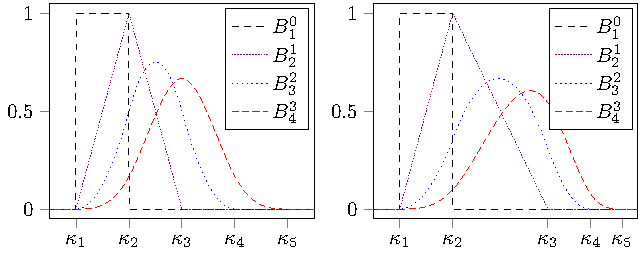
\includegraphics{graphics/pgfplots/cha2/spline-types.pdf}
	\caption[B-spline basis functions of order $l=0,1,2,3$]{B-spline basis function of order $l=0, 1, 2, 3$ given by the superscript $l$ in $B_j^l$ for equidistant (left) and non-equidistant (right) knots.}
	\label{fig:spline-types-both}
\end{figure}

The left plot shows the B-spline basis functions based on an equidistant sequence of knots. The B-spline basis function $B_1^0$ is the zero function, except for $x \in [\kappa_1, \kappa_2]$ where it is equal to 1, see~\pref{eq:Bspline_recDef1}. The B-spline basis function $B_2^1$ is the well known \emph{hat function}, being zero except for $x \in [\kappa_1, \kappa_3]$. It consists of two linear pieces, one defined from $\kappa_1$ to $\kappa_2$, the other from $\kappa_2$ to $\kappa_3$. This can be seen by expanding the recursive definition~\pref{eq:Bspline_recDef2} to

\begin{subequations} \label{eq:Bspline-BF_21}
	\begin{align}
		B_2^1(x) = a_1(x) B_1^0(x) + a_2(x) B_2^0(x)
	\end{align}
	with
	\begin{equation}
		a_1(x) = \frac{x - \kappa_1}{\kappa_2 - \kappa_1} 
	\end{equation}
	\begin{equation}
		a_2(x) = \frac{\kappa_3 - x}{\kappa_3 - \kappa_2}. 
	\end{equation}
\end{subequations}
%
Everywhere else, $B_2^1$ is equal to zero. At the joining points, the values of the linear pieces are equal. The B-spline basis function $B_3^2$ consists of three quadratic pieces, joining at the knots $\kappa_2$ and $\kappa_3$. Expanding the recursive definition shows this as

\begin{subequations}
	\begin{align}
		B_3^2(x) = a_1(x) B_1^0(x) + a_2(x) B_2^0(x) + a_3(x) B_3^0(x)
	\end{align}
	with
	\begin{equation}
		a_1(x) = \frac{x-\kappa_1}{\kappa_3 - \kappa_1} \frac{x - \kappa_1}{\kappa_2 - \kappa_1}
	\end{equation}
	\begin{equation}
		a_2(x) = \frac{x - \kappa_1}{\kappa_3 - \kappa_1} \frac{\kappa_3 - x}{\kappa_3 - \kappa_2} + \frac{\kappa_4 - x}{\kappa_4 - \kappa_2} \frac{x - \kappa_2}{\kappa_3 - \kappa_2}
	\end{equation}
	\begin{equation}
		a_3(x) = \frac{\kappa_4 - x}{\kappa_4 - \kappa_2} \frac{\kappa_4 - x}{\kappa_4 - \kappa_3}.	
	\end{equation}
\end{subequations}
%
At $\kappa_2$ and $\kappa_3$, the values of the quadratic pieces, as well as their first-order derivatives are equal. Finally, the B-spline basis function $B_4^3$ consists of 4 cubic pieces with the joining points at $\kappa_2$, $\kappa_3$ and $\kappa_4$ at which respective cubic polynomials possess equal values as well as equal first-order and second-order derivatives. Expanding the recursive definition shows this as

\begin{subequations}
	\begin{align}
		B_4^3(x) = a_1(x) B_1^0(x) + a_2(x) B_2^0(x) + a_3(x) B_3^0(x) + a_4(x) B_4^0(x)
	\end{align}
	with 
	\begin{equation}
		a_1(x) = \frac{x - \kappa_1}{\kappa_4 - \kappa_1} \frac{x - \kappa_1}{\kappa_3 - \kappa_1} \frac{x - \kappa_1}{\kappa_2 - \kappa_1}
	\end{equation}
	\begin{equation}
		a_2(x) = \frac{x - \kappa_1}{\kappa_4 - \kappa_1} \frac{x - \kappa_1}{\kappa_3 - \kappa_1} \frac{\kappa_3 - x}{\kappa_3 - \kappa_2} + \frac{x - \kappa_1}{\kappa_4 - \kappa_1} \frac{\kappa_4 - x}{\kappa_4 - \kappa_2} \frac{x - \kappa_2}{\kappa_3 - \kappa_2} + \frac{\kappa_5 - x}{\kappa_5 - \kappa_2} \frac{x - \kappa_2}{\kappa_4 - \kappa_2} \frac{x - \kappa_2}{\kappa_4 - \kappa_2}
	\end{equation}
	\begin{equation}
		a_3(x) = \frac{x - \kappa_1}{\kappa_4 - \kappa_1} \frac{\kappa_4 - x}{\kappa_4 - \kappa_2} \frac{\kappa_4 - x}{\kappa_4 - \kappa_3} + \frac{\kappa_5 - x}{\kappa_5 - \kappa_2} \frac{x - \kappa_2}{\kappa_4 - \kappa_2} \frac{\kappa_4 - x}{\kappa_4 - \kappa_3} + \frac{\kappa_5 - x}{\kappa_5 - \kappa_2} \frac{\kappa_5 - x}{\kappa_5 - \kappa_3} \frac{x - \kappa_3}{\kappa_4 - \kappa_3}
	\end{equation}
	\begin{equation}
		a_4(x) = \frac{\kappa_5 - x}{\kappa_5 - \kappa_2} \frac{\kappa_5 - x}{\kappa_5 - \kappa_3} \frac{\kappa_5 - x}{\kappa_5 - \kappa_4}.
	\end{equation}
\end{subequations}
%
The right plot in~\pref{fig:spline-types-both} shows the B-spline basis functions of the same order $l=0,1,2,3$ defined on a non-equidistant knot sequence. The shown locality, i.e. being nonzero only over a sequence of $l+2$ knots, is a very attractive feature leading to enhanced numerical properties compared to other types of splines. Some general properties of a B-spline basis function of order $l$ are summarized in the following list. Note that these properties are valid independent of the type of the knot placement.

\begin{enumerate}[(i)]
	\item A B-spline basis function consists of $l+1$ polynomial pieces of degree $l$, e.g. a cubic B-spline basis function ($l=3$) consists of 4 cubic pieces.
	\item The pieces join at $l$ inner knots.
	\item At these knots, the derivatives up to order $l-1$ are continuous.
	\item The B-spline basis function is positive on the domain spanned by $l+2$ knots, everywhere else it is zero, e.g. for $l=2$, a sequence of 4 knots is necessary.
	\item At every given $x$, only $l+1$ B-spline basis functions are nonzero.
\end{enumerate}

Using the definition of B-spline basis functions, see~\pref{eq:Bspline_recDef1} and~\pref{eq:Bspline_recDef2}, the first-order derivative of a B-spline basis function of order $l$ is given by

\begin{align} \label{eq:Bspline-bf-derivative}
	\frac{\partial}{\partial x} B_j^l(x) = l \left[\frac{1}{\kappa_j - \kappa_{j-l}} B_{j-1}^{l-1}(x) - \frac{1}{\kappa_{j+1} - \kappa_{j+1-l}} B_j^{l-1}(x) \right]
\end{align}
%
using B-spline basis functions of order $l-1$, see \cite{fahrmeir2007regression}. Higher-order derivatives are obtained by using lower order B-spline basis functions, see \cite{deBoor1978practicalGuideToSplines}. \\

As shown in~\pref{fig:spline-types-both}, the knots can either be an equidistant sequence, which facilitates the construction and estimation of the coefficients, or a non-equidistant sequence. For equidistant knots, we split the domain $[a,b]$ into $m-1$ intervals, i.e.

\begin{align} \label{eq:equidistant-knots-interval}
	h = \frac{b - a} {m - 1},
\end{align}
%
where $m$ is given by $m = d - l + 1$ and obtain the sequence

\begin{align} \label{eq:equidistant-knots-sequence}
	\kappa_j = a + h(j-1), \quad j=1, \dots, m.
\end{align} 
%
Non-equidistant knot placement can be obtained using e.g. quantile-based knots, i.e. by using the $(j-1)/(m-1)$-quantiles for $j=1, \dots, m$ of the observed inputs $x^{(1)}, \dots, x^{(n)}$ as knots. Using this approach, more knots are placed in the areas where lots of data are present. The boundary knots, i.e. $\{\kappa_{1-l}, \dots, \kappa_0\}$ on the left side and $\{\kappa_{d-l+2}, \dots, \kappa_{d+1}\}$ on the right side, are usually set to be apart from each other by at least the minimal knot distance \cite{fahrmeir2007regression}. \\

The collection of $d$ B-spline basis functions of order $l$ over a sequence of knots $K = \{\kappa_{1-l}, \kappa_{1-l+1}, \\ \dots, \kappa_{d+1}\}$ is called B-spline basis. The basis is created such that it covers the domain $[a, b]$, i.e.

\begin{align}
	\sum_{j=1}^d B_j^l(x) = 1 \ \text{for} \ x \in [a,b].
\end{align}
%
A function $f(x)$ can then be represented with a B-spline basis by 

\begin{align} \label{eq:bspline-bf-approach}
	f(x) = \sum_{j=1}^d B_j^l(x) \beta_j = \transpose{\vec{b}} \vec{\beta}_b,
\end{align}
%
using the B-spline basis functions $B_j^l(x)$ of appropriate order $l$ and the parameter vector $\transpose{\vec{\beta}}_b = [\beta_1, \dots, \beta_d] \in \mathbb{R}^{1 \times d}$. The basis functions can be given in vector notation as $\transpose{\vec{b}} = [B_1^l(x), \dots, B_d^l(x)] \in \mathbb{R}^{1 \times d}$. Using the data set $\mathcal{D} = \{(x^{(i)}, y^{(i)}), \ i=1,2, \dots, n \}$, the B-spline basis matrix for $d$ basis functions of order $l$ is given by the matrix $\vec{B}$ as

\begin{align} \label{eq:bspline-basis-matrix}
	\vec{B} = \begin{bmatrix}
				B_1^l(x^{(1)}) & \dots & B_d^l(x^{(1)})  \\
				\vdots         &       & \vdots 		 \\
				B_1^l(x^{(n)}) & \dots & B_d^l(x^{(n)})  \\
	\end{bmatrix} \in \mathbb{R}^{n \times d}.
\end{align}
%
The $n$ equations~\pref{eq:bspline-bf-approach} can then be arranged as a linear model in the form, cf.~\pref{eq:LinearModel},

\begin{align} \label{eq:Bspline-linModel}
	\vec{y} = \vec{B} \vec{\beta}_b + \vec{\epsilon}.
\end{align}
%
Once the basis matrix in~\pref{eq:bspline-basis-matrix} is given, the parameters $\vec{\beta}_b$ can be estimated using the Least Squares algorithm given in Section~\pref{subsubsec:Method-of-LS} by minimizing the objective function

\begin{align} \label{eq:Bspline-OF}
	\text{LS}(\vec{y}, \vec{\beta}_b) = \lVert \vec{y} - \vec{B} \vec{\beta}_b \rVert_2^2.	
\end{align}
%
Therefore, the estimation is computationally efficient and easy to implement since closed-form solutions exists. Further, the advanced theoretical framework of linear models can be applied to use model selection and regularization approaches as well as to calculate e.g. confidence intervals for the parameters and the prediction.

The derivative of the function $f(x)$ in~\pref{eq:bspline-bf-approach} can be calculated by summing over all $d$ B-spline basis functions and including the estimated parameters $\vec{\beta}_b$ into the B-spline basis function derivative~\pref{eq:Bspline-bf-derivative} as

\begin{align} \label{eq:Bspline-derivative}
	\frac{\partial{f(x)}}{\partial x}= \frac{\partial}{\partial x} \sum_{j}^d B_j^l(x) \beta_j = l \sum_{j}^d \frac{\beta_j - \beta_{j-1}}{\kappa_j - \kappa_{j-l}} B_{j-1}^{l-1}(x).
\end{align}
%
\begin{comment}
The second-order derivative of $f(x)$ can be given as

\begin{align} \label{eq:Bspline-2nd-derivative}
	\frac{\partial^2 {f(x)}}{\partial{x^2}}= \frac{\partial^2}{\partial{x^2}} \sum_{j=1}^d B_j^l(x) \beta_j = l^2 \sum_{j=3}^d \frac{\Delta^2 \beta_j}{(\kappa_j-\kappa_{j-l})(\kappa_{j+1} - \kappa_{j+1-l})} B_{j-2}^{l-2}(x).
\end{align}

\begin{align} \label{eq:Bspline-2nd-derivative}
	\frac{\partial^2 {f(x)}}{\partial{x^2}}= \frac{\partial^2}{\partial{x^2}} \sum_{j=1}^d B_j^l(x) \beta_j = l^2 \sum_{j=3}^d \left[\frac{\Delta \beta_j}{(\kappa_j-\kappa_{j-l})} - \frac{\Delta \beta_{j-1}}{(\kappa_{j+1} - \kappa_{j+1-l})} \right] B_{j-2}^{l-2}(x).
\end{align}
%

Here, the finite difference operators $\Delta \beta_j = \beta_j - \beta_{j-1}$ and $\Delta^2  \beta_j = \Delta(\Delta \beta_j) = \beta_j - 2\beta_{j-1} +\beta_{j-2}$ are used. 
\end{comment}
Therefore, by estimating the B-spline parameters $\vec{\beta}_b$, we also generate an estimate for the derivative of the function $f(x)$, see \cite{fahrmeir2007regression}.

B-splines of appropriate order $l > 2$ produce smooths curves, i.e. first- and second-order derivatives are continuous, where the smoothness is mostly determined by the number of basis functions $d$ used. By using a low number $d$, the curve will be quite smooth, but possess a large data error. When using a high number of basis functions $d$, the data error will be small but the variance of the curve will be large. This is an example of the bias-variance trade-off, a classical problem of regression and supervised learning, see Section~\pref{subsubsec:SPSE} and \cite{deBoor1978practicalGuideToSplines}.  

%%%%%%%%%%%%%%%%%%%%%%%%%%%%%%%%%%%%%%%%%%%%%%%%%%%%%%%%%%%%%%%%%%%%%%%%%%%%%%%%%%%%%%%%%%%%%%%%%%%%%%%%%%%%%%%%%%

\subsubsection{Tensor-Product B-Splines} \label{subsubsec:tp-splines}

Tensor-product B-splines can be regarded as the multi-dimensional extension of B-splines. We examine an example for two input dimensions $x_1$ and $x_2$. Note that tensor-product B-splines can be constructed for arbitrary dimensions using the approach given below. The tensor-product B-spline basis function is constructed by considering the product of two B-spline basis functions of orders $l_1$ and $l_2$ of respective dimension, i.e.

\begin{align}
	T_{j,r}(x_1, x_2) = B_j^{l_1}(x_1) B_r^{l_2}(x_2)
\end{align}
%
for $j \in \{1, \dots, d_1\}$ and $r \in \{1, \dots, d_2\}$. For readability, we omit the order of the tensor-product B-spline basis function since, in principle, B-spline basis functions of arbitrary, even different orders $l_1 \ne l_2$ can be combined. We then obtain the basis function representation of the tensor-product B-spline $t(x_1, x_2)$ by summing all tensor-product B-spline basis functions as

\begin{align} \label{eq:tps-basis-function-notation}
	t(x_1,x_2) = \sum_{j=1}^{d_1} \sum_{r=1}^{d_2} T_{j,r}(x_1, x_2) \beta_{j,r} 
\end{align}
%
and in vector notation we obtain

\begin{align}
	t(x_1, x_2) = \transpose{\vec{t}} \vec{\beta}_t,
\end{align}
%
with $\transpose{\vec{t}} = [T_{1,1}(x_1, x_2), \dots, T_{d_1,1}(x_1, x_2), \dots, T_{1,d_2}(x_1, x_2), \dots, T_{d_1,d_2}(x_1, x_2)] \in \mathbb{R}^{1 \times d_1d_2}$ and the corresponding vector of parameters $\transpose{\vec{\beta}}_t = [\beta_{1,1}, \dots, \beta_{d_1,1}, \dots, \beta_{1,d_2}, \dots, \beta_{d_1, d_2}] \in \mathbb{R}^{1 \times d_1d_2}$. For any set of data 

\begin{align} \label{eq:data-2d}
	\mathcal{D} = \{ (x^{(i)}_{1}, x^{(i)}_{2}, y^{(i)} ), \ i=1,2, \dots, n\}, 
\end{align}
%
the tensor-product B-spline basis matrix for $d_1$ and $d_2$ basis functions in the respective dimensions is given by the matrix $\vec{T}$ as

\begin{align} \label{eq:tp-bspline-basis-matrix}
	\vec{T} = \begin{bmatrix}
		T_{1,1}(x_1^{(1)}, x_2^{(1)}) & \dots & T_{d_1,d_2}(x_1^{(1)}, x_2^{(1)})  \\
		\vdots         &       & \vdots 		 \\
		T_{1,1}(x_1^{(n)}, x_2^{(n)}) & \dots & T_{d_1,d_2}(x_1^{(n)}, x_2^{(n)})  \\
	\end{bmatrix} \in \mathbb{R}^{n \times d_1d_2}.
\end{align}
%	
The relationship between the tensor-product B-spline basis matrix $\vec{T}$ and the B-spline basis matrices $\vec{B}_1$ and $\vec{B}_2$ is then given as

\begin{align}
	\vec{T} = \vec{B}_2 \odot \vec{B}_1,
\end{align}
%
where $\odot$ indicates the use of the row-wise Kronecker product, see~\pref{apx:AppendixKroneckerRowWise}, $\vec{T} \in \mathbb{R}^{n \times d_1 d_2}$ denotes the tensor-product B-spline basis matrix, $\vec{B}_1 \in \mathbb{R}^{n \times d_1}$ is the B-spline basis matrix for dimension $x_1$ and $\vec{B}_2 \in \mathbb{R}^{n \times d_2}$ denotes the B-spline basis matrix for dimension $x_2$ \cite{fahrmeir2007regression}.  

We can now model a two dimensional function using the data set $\mathcal{D}$ in~\pref{eq:data-2d} similar to~\pref{eq:Bspline-linModel} as linear model of the form

\begin{align} \label{eq:tps-matrix-notation}
	\vec{y} = \vec{T} \vec{\beta}_t + \vec{\epsilon},
\end{align}
%
with the tensor-product B-spline basis matrix $\vec{T} \in \mathbb{R}^{n \times d_1 d_2}$ according to~\pref{eq:tp-bspline-basis-matrix} and the parameter vector $\transpose{\vec{\beta}}_t \in \mathbb{R}^{1 \times d_1 d_2}$. Once the basis matrix in~\pref{eq:tp-bspline-basis-matrix} is given, the parameters $\vec{\beta}_t$ can be estimated using the Least Squares algorithm given in Section~\pref{subsubsec:Method-of-LS} by minimizing the objective function 

\begin{align}
	\text{LS}(\vec{y}, \vec{\beta}_t) = \lVert \vec{y} - \vec{T} \vec{\beta}_t \rVert_2^2.
\end{align}
%
This approach can in theory be repeated for as many input dimensions as required. In practice, modeling more than two input dimensions using tensor-product B-splines becomes infeasible because of the exponential increase of basis functions and therefore parameters to estimate. 


\subsubsection{Additive Regression} \label{subsubsec:STAR}

To circumvent the latter problem, we now assume the restrictive structure of additive models, see \cite{fahrmeir2007regression}, given by

\begin{align} \label{eq:addRegBaseEquation}
	f(x_1, \dots, x_q) = f_1(x_1) + \dots + f_q(x_q).
\end{align}
%
Hence, we use one function $f_i(x_i)$ per input dimension $x_i$. For some given data set $\mathcal{D} = \{ (x^{(ii)}_{1}, \dots, x^{(ii)}_{q}, y^{(ii)} ), \ ii=1,2, \dots, n\}$, by using a B-spline for each function $f_i(x_i)$ we obtain a linear model

\begin{align} \label{eq:addRegBaseEquation-as-linModel}
	f_i(\vec{x}_i) = \vec{B}_i \vec{\beta}_{b_i},
\end{align}
%
where $\vec{B}_i \in \mathbb R^{n \times d_i}$ is the B-spline basis matrix using $d_i$ B-spline basis functions for $i=1,2,\dots, q$, $\transpose{\vec{x}}_i = [x_i^{(1)}, \dots, x_i^{(n)}] \in \mathbb{R}^{1 \times n}$ is the data vector of input dimension $i$ and $\vec{\beta}_{b_i} \in \mathbb R^{d_i}$ are the parameters to estimate. This leads to the model structure 

\begin{align} 
	\vec{y} =  \vec{B}_1 \vec{\beta}_{b_1} + \dots + \vec{B}_q \vec{\beta}_{b_q} + \vec{\epsilon},
\end{align}
%
which can be written as linear model by concatenation of the B-spline basis matrices and parameter vectors as 

\begin{align} \label{eq:STAR-single-block-diag}
	\vec{y} = \vec{X} \vec{\beta} + \vec{\epsilon}= 
				\begin{bmatrix}
					\vec{B}_1, \dots, \vec{B}_q 
				\end{bmatrix}
			    \begin{bmatrix}
					\vec{\beta}_{b_1} \\ 
					\vdots \\
					\vec{\beta}_{b_q} 
				\end{bmatrix} + \vec{\epsilon},
\end{align}
%
with the matrix $\vec{X} \in \mathbb{R}^{n \times d_{total}}$, the parameter vector $\vec{\beta} \in \mathbb{R}^{d_{total}}$ and $d_{total} = \sum_{i=1}^q d_i$ as the total number of parameters. The model~\pref{eq:STAR-single-block-diag} does not contain interaction terms between inputs. Nevertheless, these can be easily introduced for two dimensions using tensor-product B-splines without an overflowing increase in the number of coefficients. We can then write the additive model with interaction terms as 

\begin{align} \label{eq:addRegBaseEquation-with-interaction}
	f(x_1, \dots, x_q) = f_1(x_1) + \dots + f_q(x_q) + f_{1,2}(x_1, x_2) + \dots + f_{q-1, q}(x_{q-1},x_q).
\end{align}
%
Hence, we use one function $f_i(x_i)$ per input dimension and per interaction term. Using a tensor-product B-spline $t_{j,r}(x_j, x_r)$ for each interaction term, we obtain the model

\begin{align} \label{eq:STAR}
	\vec{y} = \vec{B}_1 \vec{\beta}_{b_1} + \dots + \vec{B}_q \vec{\beta}_{b_q} + \sum_{j=1}^{q-1} \sum_{r>j}^{q} \vec{T}_{j, r} \vec{\beta}_{t_{j, r}} + \vec{\epsilon},
\end{align}
%
using the tensor-product B-spline basis matrices $\vec{T}_{j,r} \in \mathbb{R}^{n \times d_j d_r}$ and the parameter $\vec{\beta}_{t_{j, r}} \in \mathbb{R}^{d_j d_r}$. Using the notation in~\pref{eq:STAR}, the theoretical framework of linear models can be applied to the additive regression model, since~\pref{eq:STAR} can be formulated as linear model yielding

\begin{align} \label{eq:STAR-block-diag}
	\vec{y} = \vec{X} \vec{\beta} + \vec{\epsilon} = 
	\begin{bmatrix}
		\vec{B}_1 , \dots , \vec{B}_q, \vec{T}_{1,2}, \dots, \vec{T}_{q-1, q}    
	\end{bmatrix} \begin{bmatrix} \vec{\beta}_{b_1} \\ 
								  \vdots \\ 
								  \vec{\beta}_{b_q} \\ 
								  \vec{\beta}_{t_{1,2}} \\ 
								  \vdots \\ 
								  \vec{\beta}_{t_{q-1, q}} \\
	\end{bmatrix} + \vec{\epsilon},
\end{align}
%
with $\vec{X} \in \mathbb{R}^{n \times d_{total}}$ as design matrix, $\vec{\beta} \in \mathbb{R}^{d_{total}}$ as parameter vector and $d_{total} = \sum_{i=1}^q d_i + \sum_{j=1}^{q-1} \sum_{r>j}^q d_j d_r$ as the total number of parameters in the model. Hence, the parameters can be calculated efficiently using the Least Squares (LS) algorithm, see Section~\pref{subsubsec:Method-of-LS}. Further, the assumptions given in~\pref{sec:LinModel} on the error term, as well as on the model function are used.

Note that additive models are not limited to be used with B-splines. We can also include the linear model given in~\pref{sec:LinModel}. For 2 input dimensions $x_1$ and $x_2$, we then obtain a model of the form

\begin{align}
	\vec{y} = \vec{X} \vec{\beta} + \vec{B}_1 \vec{\beta}_{b_1} + \vec{B}_2 \vec{\beta}_{b_2} + \vec{T}_{1,2} \vec{\beta}_{t_{1,2}},
\end{align}
%
where $\vec{X} \in \mathbb{R}^{n \times 2}$ is the design matrix of the linear model, $\vec{B}_1$ and $\vec{B}_2$ are the respective B-spline basis matrices and $\vec{T}_{1,2}$ is the tensor-product B-spline matrix. 

%%%%%%%%%%%%%%%%%%%%%%%%%%%%%%%%%%%%%%%%%%%%%%%%%%%%%%%%%%%%%%%%%%%%%%%%%%%%%%%%%%%%%%%%%%%%%%%%%%%%%%%%%%%%%%%%%%
\subsection{P-Splines} \label{subsec:p-splines}

P-splines combine the concepts of B-spline basis functions and regularization to produce sufficiently smooth function estimations. A function is said to be smooth if its second-order derivative is continuous. Therefore, a penalty of the form 

\begin{align} \label{eq:wiggliness-penalty}
	\lambda \cdot \int \left(f''(x)\right)^2 \,\mathrm{d}x
\end{align}
%
is typically introduced to penalize the curvature of a function which is measured by its second-order derivative \cite{osullivan1986penalties}. The penalty is weighted by the so-called \emph{smoothing parameter} $\lambda$. This yields the penalized least squares objective function, cf. Section~\pref{subsec:Regularization}, as

\begin{align} \label{eq:P-splines-OF-base}
	\text{PLS}(\vec{y}, \vec{\beta}; \lambda) = \lVert \vec{y} - \vec{B} \vec{\beta}_b \rVert_2^2 + \lambda \int \left(f''(x)\right)^2 \,\mathrm{d}x
\end{align}
%
using the B-spline basis matrix $\vec{B} \in \mathbb{R}^{n \times d}$ for some data $\mathcal{D}=\{(x^{(i)}, y^{(i)}), \ i=1,2,\dots,n\}$. Inserting the B-spline basis function formulation~\pref{eq:bspline-bf-approach}, using order $l$ and $d$ basis functions, into~\pref{eq:wiggliness-penalty} results in

\begin{align} \label{eq:p-spline-approx-deriv}
	\begin{split}
		\int \left(f''(x)\right)^2 \,\mathrm{d}x &= \int \left(\sum_{j=1}^d B''_j(x) \beta_j \right)^2 \,\mathrm{d}x \\
						     &= \int \sum_{j=1}^d \sum_{r=1}^d \beta_j \beta_r B''_j(x) B''_r(x) \,\mathrm{d}x \\
						     &= \transpose{\vec{\beta}} \vec{K} \vec{\beta},
	\end{split}
\end{align}
% 
with the penalty matrix $\vec{K}[j,r] = \int B''_j(x) B''_r(x) \,\mathrm{d}x$ as a matrix of dimension $\mathbb{R}^{d \times d}$. The entries of $\vec{K}$ are given by the integrated products of the second-order derivatives of the B-spline basis functions $B_j(x)$ and $B_r(x)$. For readability, the order $l$ is omitted. These second-order derivatives can be obtained by using the derivative properties of B-spline basis functions, see \cite{fahrmeir2007regression}. 

Eilers and Marx proposed in \cite{eilers1996flexible} to base the penalty on finite differences of higher order of the parameters of adjacent B-spline basis functions which circumvents the direct calculation of the second-order derivative and the integral. Hence, the complexity is reduced from $n$, the number of data points to evaluate the integral on, to $d$, the number of parameters \cite{eilers1996flexible}. The squared second-order finite difference gives a good discrete approximation of the integral of the squared second-order derivative in~\pref{eq:wiggliness-penalty}, i.e.

\begin{align} \label{eq:wiggliness-finite-diff-approx}
	\sum_{j=3}^d \left(\Delta^2 \beta_j\right)^2 \propto \int \left(f''(x)\right)^2 \,\mathrm{d}x
\end{align}
%
where $\Delta^2 \beta_j$ is defined as 

\begin{align} \label{eq:2nd-order-finite-diff}
	\begin{split}
		\Delta^2 \beta_j &= \Delta(\Delta \beta_j) \\
						 &= \Delta( \beta_j - \beta_{j-1}) \\
						 &= \beta_j - 2\beta_{j-1} + \beta_{j-2}.
	\end{split}
\end{align}
%
In matrix form,~\pref{eq:2nd-order-finite-diff} may be given as

\begin{align} \label{eq:2nd-order-finite-diff-matrix}
	\vec{D}_2 \vec{\beta}_b = 
					\begin{bmatrix} 
						1& -2      & 1&      \\  
						 &  \ddots & \ddots  & \ddots \\ 
						 &         &   1     & -2 & 1 
					\end{bmatrix} \begin{bmatrix}
						\beta_1 \\
						\vdots \\
						\beta_d
				\end{bmatrix},
\end{align}
%
with $\vec{D}_2 \in \mathbb{R}^{(d-2) \times d}$. Applying the matrix form of the second-order finite difference operator~\pref{eq:2nd-order-finite-diff-matrix} into~\pref{eq:wiggliness-finite-diff-approx} yields

\begin{align}
	\lambda \sum_{j=3}^d \left(\Delta^2 \beta_j \right)^2 = \lambda \transpose{\vec{\beta}}_b \transpose{\vec{D}}_2 \vec{D}_2 \vec{\beta}_b = \lambda \transpose{\vec{\beta}}_b \vec{K} \vec{\beta}_b.
\end{align}
%
We then obtain the objective function to minimize as

\begin{align} \label{eq:P-spline-final-OF}
	\text{PLS}(\vec{y}, \vec{\beta}; \lambda) = \lVert \vec{y} - \vec{B} \vec{\beta}_b \rVert_2^2 + \lambda \transpose{\vec{\beta}}_b \vec{K} \vec{\beta}_b,
\end{align}
%
which is equivalent to the objective function of Ridge regression, cf. Section~\pref{subsec:Regularization}, for the special choice of $\vec{K}$ given by $\vec{K} = \transpose{\vec{D}}_2 \vec{D}_2 \in \mathbb{R}^{d \times d}$. As in Ridge regression, the smoothness parameter $\lambda$ plays a critical role. For $\lambda \rightarrow 0$, the P-spline approaches the underlying B-spline since the penalty term in~\pref{eq:P-spline-final-OF} goes to $0$. For $\lambda \rightarrow \infty$, the P-spline approaches a polynomial model. The order of the polynomial is given by the order of the finite difference penalty, e.g. for second-order finite difference penalty, we penalize the discrete approximation of the second-order derivative leading to a linear function, because for these, the second-order derivative is equal to zero. Note that higher-order difference penalties are also possible.

The main advantage of P-splines is their easy set up by replacing the integral of the squared second-order derivative of the B-spline basis functions with the squared second-order finite differences of parameters of adjacent B-spline basis functions. This reduces the computational complexity and allows faster training and evaluation. Hence, P-splines are widely used in practice \cite{eilers1996flexible}. \\

A similar penalty term for tensor-product B-splines can be constructed using the Kronecker product.  Recall the definition of a tensor-product B-spline given in~\pref{eq:tps-basis-function-notation} and~\pref{eq:tps-matrix-notation}.


The spatial alignment of the B-spline basis functions and the corresponding parameters of the two-dimensional tensor-product B-spline needs to be incorporated by the definition of the term \emph{adjacent parameters}. An example for these adjacent parameters, also called spatial neighborhood, is taken from \cite{fahrmeir2007regression} and given in~\pref{fig:tps-neighborhood}. Here, we choose the parameters left and right, i.e. $\beta_{j, r-1}$ and $\beta_{j, r+1}$, as well as above and below, i.e. $\beta_{j-1,r}$ and $\beta_{j+1, r}$, as spatial neighborhood for $\beta_{j,r}$. 

\begin{figure}[H]
	\centering	
	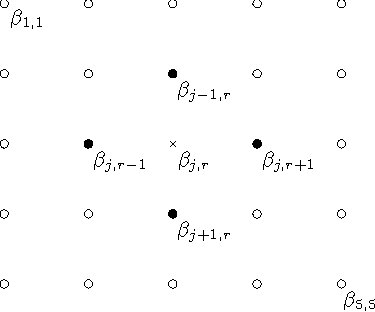
\includegraphics{graphics/pgfplots/cha2/tps-spatial-neighborhood.pdf}
	\caption{Spatial neighborhood or adjacent parameters for a tensor-product B-spline.}
	\label{fig:tps-neighborhood}
\end{figure}
%
We now use the concepts of P-splines in both dimensions and penalize the integral of the squared Hessian of the tensor-product B-spline, see~\pref{eq:wiggliness-penalty}, by a higher-order finite difference approximation in both dimensions. Using second-order finite differences as in~\pref{eq:wiggliness-finite-diff-approx} leads to the following definition of the penalty term

\begin{align}
	\left[ \sum_{j=3}^{d_1} \sum_{r=1}^{d_2} (\Delta_1^2 \beta_{j,r})^2 + \sum_{j=1}^{d_1} \sum_{r=3}^{d_2} (\Delta_2^2 \beta_{j,r})^2 \right] \propto \iint \left(f''(x_1, x_2) \right)^2 \,\mathrm{d}x_1 \,\mathrm{d}x_2
\end{align}
%
as discrete approximation of the integral of the squared Hessian of the tensor-product B-spline. The first term on the left side calculates the "row-wise" squared second-order differences, i.e. in direction $x_1$, using

\begin{align} \label{eq:row-wise-diff-operator}
	\Delta_1^2 \beta_{j,r} = \beta_{j,r} - 2\beta_{j-1,r} + \beta_{j-2,r} 
\end{align}
%
and the second term on the left side calculates the "column-wise" squared second-order differences, i.e. in direction $x_2$, using

\begin{align} \label{eq:col-wise-diff-operator}
	\Delta_2^2 \beta_{j,r} = \beta_{j,r} -2\beta_{j,r-1} + \beta_{j,r-2}.
\end{align}
%
The subscript for $\Delta$ in~\pref{eq:row-wise-diff-operator} and~\pref{eq:col-wise-diff-operator} indicates the direction of the finite differences. Using the matrix form of the second-order finite difference operator and the Kronecker product, see~\pref{apx:AppendixKronecker}, as well as the parameter vector $\vec{\beta}_t \in \mathbb{R}^{d_1 d_2 \times 1}$, we can then write the "row-wise" penalty as

\begin{align} \label{eq:row-wise-penalty}
	\transpose{\vec{\beta}}_t \transpose{(\vec{I}_{d_2} \otimes \vec{D}_{1,2})} (\vec{I}_{d_2} \otimes \vec{D}_{1,2}) \vec{\beta}_t = \sum_{j=3}^{d_1} \sum_{r=1}^{d_2} \left(\Delta_1^2 \beta_{j,r} \right)^2
\end{align}
%
and the "column-wise" penalty as

\begin{align} \label{eq:col-wise-penalty}
	\transpose{\vec{\beta}}_t \transpose{(\vec{D}_{2,2} \otimes \vec{I}_{d_1})} (\vec{D}_{2,2} \otimes \vec{I}_{d_1}) \vec{\beta}_t = \sum_{j=1}^{d_1} \sum_{r=3}^{d_2} \left(\Delta_2^2 \beta_{j,r} \right)^2
\end{align}
%
using the identity matrices $\vec{I}_{d_1} \in \mathbb{R}^{d_1 \times d_1}$ and $\vec{I}_{d_2} \in \mathbb{R}^{d_2 \times d_2}$ and the second-order difference matrices $\vec{D}_{1,2} \in \mathbb{R}^{(d_1 - 2) \times d_1}$ and $\vec{D}_{2,2} \in \mathbb{R}^{(d_2 - 2) \times d_2}$, cf.~\pref{eq:2nd-order-finite-diff-matrix}. The first subscript of $\vec{D}$ indicates the direction of the finite differences and the second subscript indicates the use of the second-order finite differences. Summing up both penalties leads to a formulation similar to~\pref{eq:P-spline-final-OF} given by

\begin{align} \label{eq:TP-P-spline-final-OF}
	\text{PLS}(\vec{y}, \vec{\beta}_t; \lambda) = \lVert \vec{y} - \vec{T} \vec{\beta}_t \rVert_2^2 + \lambda \transpose{\vec{\beta}}_t \vec{K} \vec{\beta}_t,
\end{align}
%
with the tensor-product B-spline basis matrix $\vec{T} \in \mathbb{R}^{n \times d_1 d_2}$, the smoothing parameter $\lambda$ and the penalty matrix $\vec{K}$ given by

\begin{align}
	\vec{K} = \left[ \transpose{(\vec{I}_{d_2} \otimes \vec{D}_{1,2})} (\vec{I}_{d_2} \otimes \vec{D}_{1,2}) + \transpose{(\vec{D}_{2,2} \otimes \vec{I}_{d_1})} (\vec{D}_{2,2} \otimes \vec{I}_{d_1}) \right] \in \mathbb{R}^{d_1 d_2 \times d_1 d_2}.
\end{align}